\documentclass[main.tex]{subfiles}


\begin{document}


\subsection{The frameshifting pseudoknot competes with the long-range interaction}

We refined the model of the long-range interaction using the mutational profiling data from both clusters that corresponded to this interaction forming (Figure \ref{tiles}c, d).
We predicted the structure of a 1,799 nt segment of the genome centered on the long-range interaction using RNAstructure Fold \cite{Mathews2004a}.
The minimum free energy structure (Figure \ref{lnas}) contained not only the two inner stems of the FSE-arch (LS1 and LS2a/b) but also two additional stems that were not part of the original FSE-arch model~\cite{Ziv2020} (LS3a/b and LS4).
The structure also contained the alternative stem 1 (AS1) that we had previously discovered~\cite{Lan2022}, which encircles the attenuator hairpin (AH)~\cite{Su2005}.
Because we had collected DMS-MaPseq data on both ends of LS3a/b, but only the 5' end of LS4, we focused on LS3a/b.

To our surprise, LS2b, LS3a/b, and LS4 of the new model penetrate into structures within the FSE pseudoknot that is widely thought to stimulate frameshifting -- LS2b overlaps with PS2, LS3 with PS3, and LS4 with PS1.
We had previously shown that AS1 also overlaps with and seems to outcompete PS1~\cite{Lan2022}.
If these stems existed, then they would be mutually exclusive with the FSE pseudoknot, which suggests that the long-range interaction could inhibit the formation of the pseudoknot and possibly regulate the rate of frameshifting.

Thus, we verified these structures of the long-range interaction using SEARCH-MaP.
We performed SEARCH-MaP on the same 1,799 nt segment for which we had predicted the structure, this time with shorter LNA/DNA mixmer ASOs (15-20 nt) to reach single-stem precision.
Each ASO targeted a single stem in the downstream portion of the interaction, and we measured the change in DMS reactivities of the FSE.
ASOs targeting the 3' sides of LS1 and LS2a perturbed the DMS reactivities in exactly the expected locations on the 5' sides (Figure \ref{lnas}b).
Binding an ASO to the 3' side of LS2b caused a larger perturbation with more off-target effects, likely because this stem overlaps with stem 2 of the pseudoknot (PS2), so blocking it with an ASO could promote pseudoknot formation.
Blocking LS3b also resulted in a main effect around the intended location, with one off-target effect upstream, suggesting that there may be another RNA--RNA interaction with the pseudoknot and this upstream region.
These results show that stems LS1, LS2a/b, and LS3b in the refined model of the long-range interaction do exist and can be detected with SEARCH-MaP -- cleanly if the stem does not interact with anything else, otherwise with off-target effects.

Assuming that all stems in Figure \ref{lnas}a do exist, we found that there are six possible structure models resulting from all possible combinations of non-overlapping stems (Figure \ref{lnas}c).
We ordered these models from most long-range character (A) to most pseudoknot-like character (F).
We then determined whether each model actually exists in the ensemble and estimated its proportion.

We found that our no-ASO control clustered reproducibly up to 6 clusters (SFIG).
For each cluster, we found how well it agreed with each structure model by calculating the area under the receiver operating characteristic curve (AUC-ROC).
We graph the results as a heatmap with clusters on the x-axis, in order of and their widths indicating their proportions in the ensemble, and the models on the y-axis.
We consider a cluster and model to be consistent with each other if the AUC-ROC is at least 0.90, and explicitly print all such AUC-ROC values.
We found that model C -- in which AS1 folds along with stems PS2 and PS3 of the pseudoknot -- was consistent with three clusters representing 52\% of the ensemble (Figure \ref{lnas}d, top).
Model A -- where the full long-range interaction forms -- was consistent with one cluster (20\%).
No clusters were consistent with the pseudoknot (Model F); the least-abundant cluster (7\%) came close with an AUC-ROC of 0.88.
The remaining cluster (21\%) was not even close to being consistent with any model, suggesting that there are still other structures in the ensemble besides those in Figure \ref{lnas}c.

These results suggested to us that the primary competitors of the pseudoknot are AS1 and LS2b, since both are present in the most abundant model, C (52\%), while LS3 and LS4 fold in model A, which is only 20\% of the ensemble.
We thus reasoned that if the long-range interaction does actually compete with the pseudoknot, then blocking AS1 and LS2b simultaneously should allow the pseudoknot to fold, while blocking either would have a much smaller effect on the pseudoknot.
To test this hypothesis, we repeated the above experiment while adding an ASO targeting either AS1 or just the part of LS2b that overlaps with the pseudoknot, or both ASOs together.
Blocking AS1 (Figure \ref{lnas}d, left) reduced the proportion of clusters consistent with AS1 (Models A, B, and C) from 72\% to 16\%, as expected; it also resulted in two clusters consistent with the pseudoknot (56\% total) and one cluster (20\%) consistent with Model D, which includes PS1.
Blocking the part of LS2b that seems to overlap with PS2 (Figure \ref{lnas}d, right) eliminated Model A but not Model C (as expected, since Model A includes LS2b, while Model C does not), and also produced one cluster (13\%) that was consistent with the pseudoknot.
Blocking both AS1 and LS2b together (Figure \ref{lnas}d, bottom) forced the entire ensemble into the pseudoknot state, with 87\% of the ensemble highly consistent with Model F (AUC-ROC = 0.97) and the remaining 13\% still somewhat consistent (AUC-ROC = 0.87).
Thus, we conclude that the long-range interaction -- particularly LS2b -- along with AS1, does compete with the pseudoknot.

\begin{figure}[ht]
	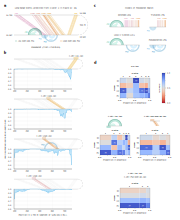
\includegraphics[width=\textwidth]{../MainFigures/lnas/lnas.pdf}
	\caption{}
	\label{lnas}
\end{figure}

\end{document}
